\documentclass[border=4pt]{standalone}

\usepackage[T1]{fontenc}
\usepackage[utf8]{inputenc}
\usepackage{amsmath}
\usepackage{xcolor}
\usepackage{tikz}
\usetikzlibrary{positioning, calc, arrows.meta, backgrounds}

\definecolor{shapedc}{RGB}{233,138,46}   % dense / shaped  : orange
\definecolor{winc}{RGB}{76,160,90}        % sparse / win-loss : green

\begin{document}

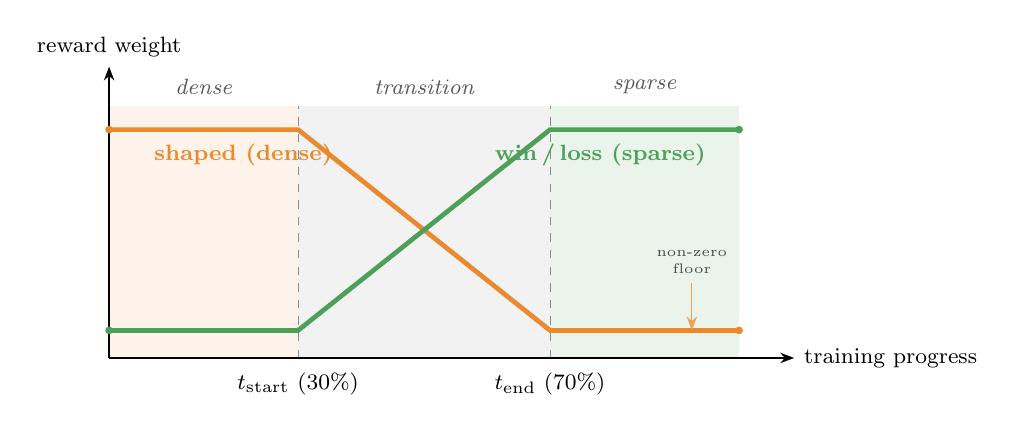
\begin{tikzpicture}[font=\small, >={Stealth[length=5pt]}]

% plot area: x in [0,8], y in [0,3.2]; t_start=30%->x=2.4, t_end=70%->x=5.6

%% ── phase bands (background) ─────────────────────────────────────
\begin{scope}[on background layer]
  \fill[shapedc!10] (0,0)   rectangle (2.4,3.2);
  \fill[black!5]    (2.4,0) rectangle (5.6,3.2);
  \fill[winc!12]    (5.6,0) rectangle (8,3.2);
\end{scope}

%% ── phase boundaries ─────────────────────────────────────────────
\draw[dashed, black!45] (2.4,0) -- (2.4,3.2);
\draw[dashed, black!45] (5.6,0) -- (5.6,3.2);

%% ── phase captions (top of each band) ────────────────────────────
\node[font=\footnotesize\itshape, text=black!65] at (1.2,3.44) {dense};
\node[font=\footnotesize\itshape, text=black!65] at (4.0,3.44) {transition};
\node[font=\footnotesize\itshape, text=black!65] at (6.8,3.44) {sparse};

%% ── axes ─────────────────────────────────────────────────────────
\draw[->, line width=0.6pt] (0,0) -- (8.7,0) node[right, font=\footnotesize] {training progress};
\draw[->, line width=0.6pt] (0,0) -- (0,3.7) node[above, font=\footnotesize] {reward weight};

%% ── weight curves ────────────────────────────────────────────────
\draw[shapedc, line width=1.7pt] (0,2.9) -- (2.4,2.9) -- (5.6,0.35) -- (8,0.35);
\draw[winc,    line width=1.7pt] (0,0.35) -- (2.4,0.35) -- (5.6,2.9) -- (8,2.9);
% endpoint markers
\foreach \p in {(0,2.9),(8,0.35)}{\fill[shapedc] \p circle(1.4pt);}
\foreach \p in {(0,0.35),(8,2.9)}{\fill[winc] \p circle(1.4pt);}

%% ── curve labels (where each weight is high) ─────────────────────
\node[shapedc, font=\footnotesize\bfseries, anchor=west] at (0.45,2.58) {shaped (dense)};
\node[winc,    font=\footnotesize\bfseries, anchor=east] at (7.7,2.58) {win\,/\,loss (sparse)};

%% ── floor annotation ─────────────────────────────────────────────
\draw[<-, shapedc!80, line width=0.5pt] (7.4,0.35) -- (7.4,0.95)
  node[above, font=\tiny, text=black!70, align=center] {non-zero\\floor};

%% ── t markers ────────────────────────────────────────────────────
\node[below, font=\footnotesize] at (2.4,-0.07) {$t_{\text{start}}$ (30\%)};
\node[below, font=\footnotesize] at (5.6,-0.07) {$t_{\text{end}}$ (70\%)};

\end{tikzpicture}

\end{document}
